
\section{Central tracking}

\subsection{Silicon microstrip tracker}

%%%%%% SLIDE
\begin{frame}{\textcolor{Goldenrod}{Silicon Microstrip Tracker}}
  \begin{overlayarea}{\textwidth}{\textheight}
    \begin{figure}[h]
      \centering
      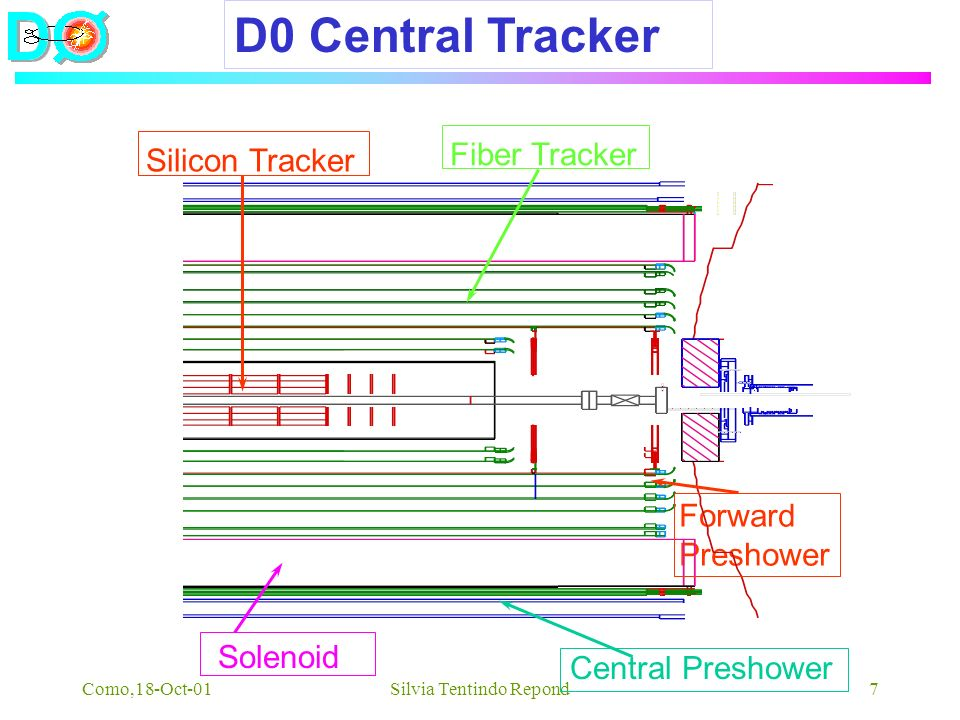
\includegraphics[height=0.5\textheight]{./Images/08_CT}
    \end{figure}

    \itt[<only@+>]
  \item
    A silicon microstrip tracker (SMT) and a central fiber tracker
    (CFT) surrounded by a solenoidal magnet

  \item
    the primary interaction vertex resolution of about $35 \mu m $
    along the beamline $\to$ \alert{ good measurement of lepton $p_T$, jet
      transverse energy ($E_T$ ), and missing transverse energy
      $\slashed{E_T}$. }\\
    \textcolor{blue}{{\small b-quark jets tagging with an impact parameter resolution of better
      than $15 \mu m$ in $r-phi$}}
    \note{for particles with transverse momentum $p_T
      > 10 GeV/c$ at $\eta = 0$.}
    \tti
  \end{overlayarea}
\end{frame}


%%%%%% SLIDE
\begin{frame}{\textcolor{Goldenrod}{Silicon Microstrip Tracker}}
  \begin{overlayarea}{\textwidth}{\textheight}
    \begin{figure}[h]
      \centering
      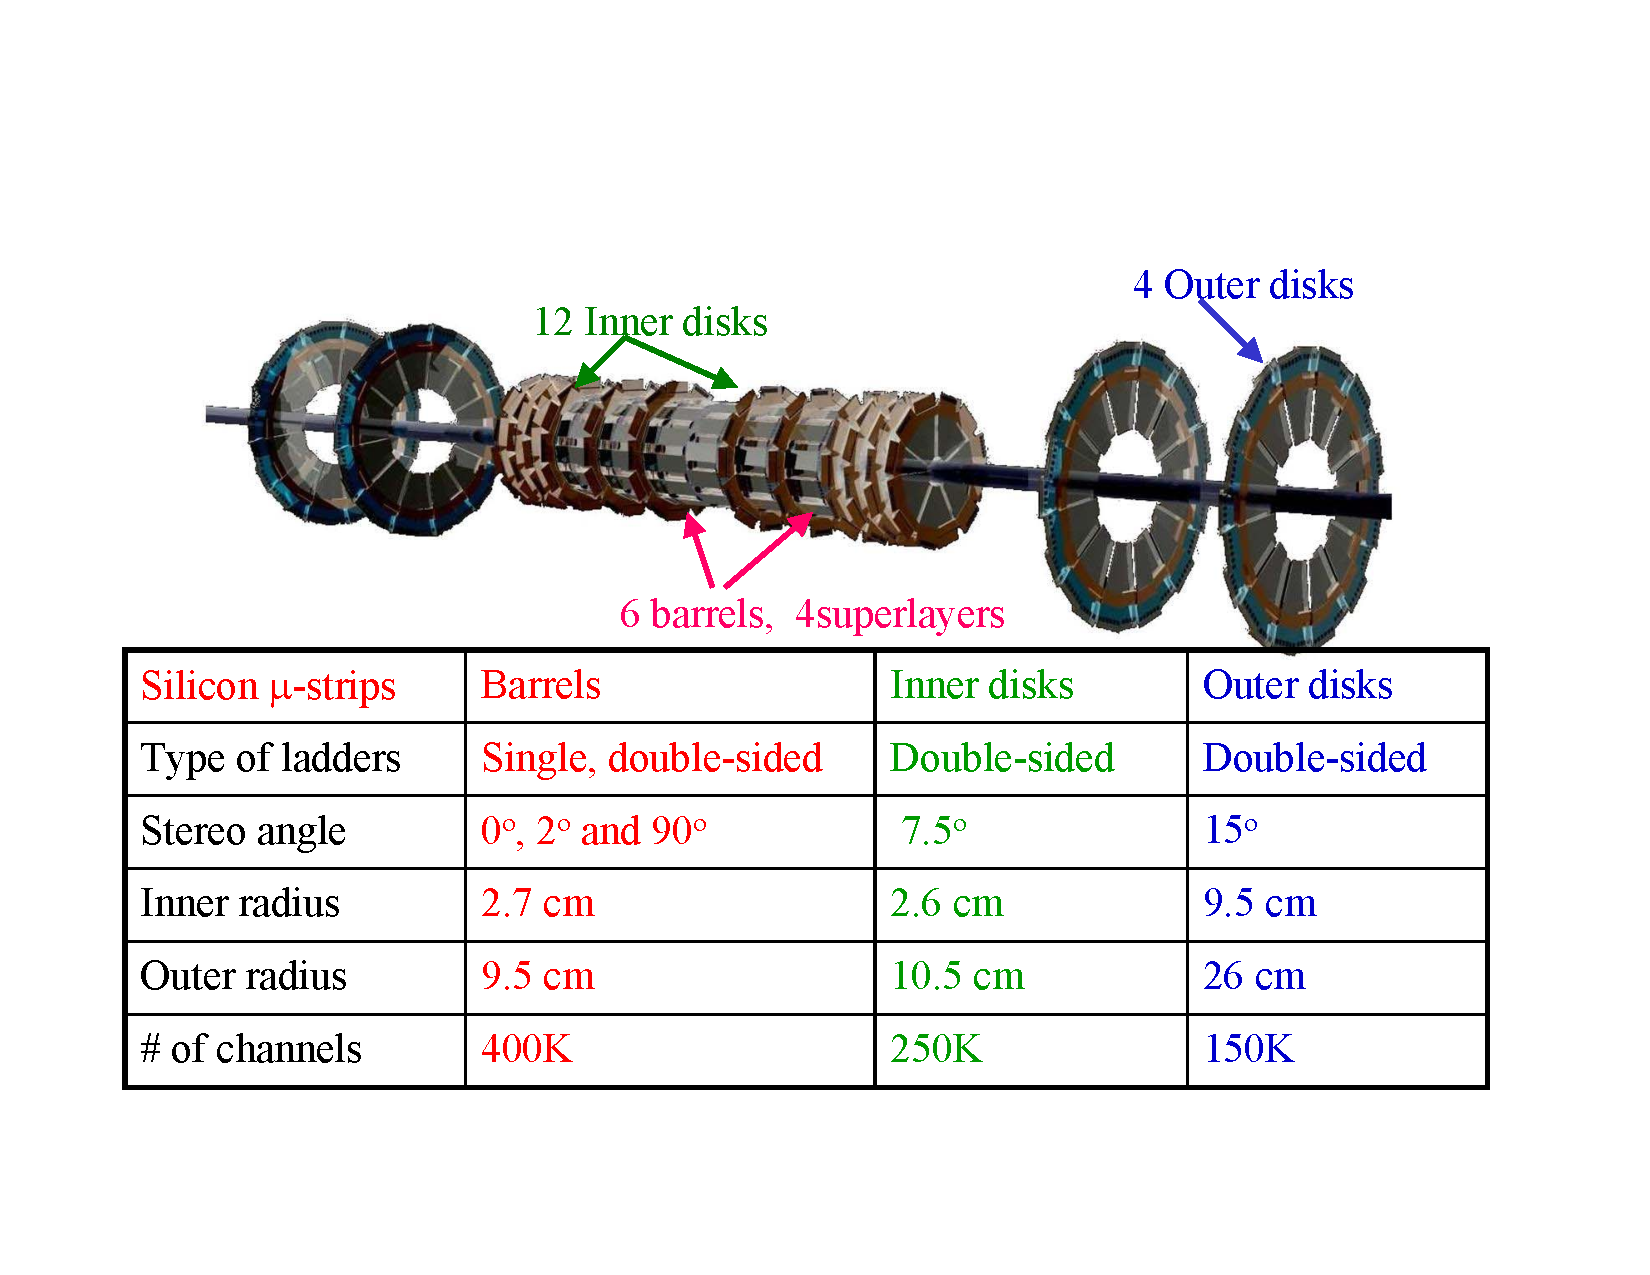
\includegraphics[height=0.4\textheight]{./Images/09_SMT}
    \end{figure}

    \itt[<only@+>]
  \item
    
 \item The SMT provides both tracking and vertexing over nearly the
   full $\eta$ coverage of the calorimeter and muon systems.
   
 \item The barrel detectors primarily measure the $r-phi$ coordinate and
   the disk detectors measure $r-z$ as well as $r-\phi$.

   
 \note{Sensor ladder assemblies were designed for low mass, pre- cise
   alignment, and good thermal performance. With the exception of the
   DSDM ladders, which use a single 12-cm sensor, ladders were
   constructed us- ing two 6-cm sensors.}
 
 \note{The SMT uses a combination of single-sided (SS), double-sided
   (DS), and double-sided double-metal (DSDM) technologies.}
 
 \note{The detector has six barrels in the central region. Each barrel
   has four silicon readout layers. The silicon modules installed in
   the barrels are called “ladders.” Layers 1 and 2 have twelve
   ladders each; layers 3 and 4 have twenty-four ladders each, for a
   total of 432 ladders.}
 
 \note{There are 144 F-wedges and 96 full H-wedges in the tracker;
   each side of a wedge (upstream and downstream) is read out
   independently. There is a grand total of 912 readout modules, with
   792,576 channels.}
 \tti
\end{overlayarea}
\end{frame}

%%%%%% SLIDE
\begin{frame}{\textcolor{Goldenrod}{Silicon Microstrip Tracker: Operation}}
  \begin{overlayarea}{\textwidth}{\textheight}
    \begin{figure}[h]
      \centering
      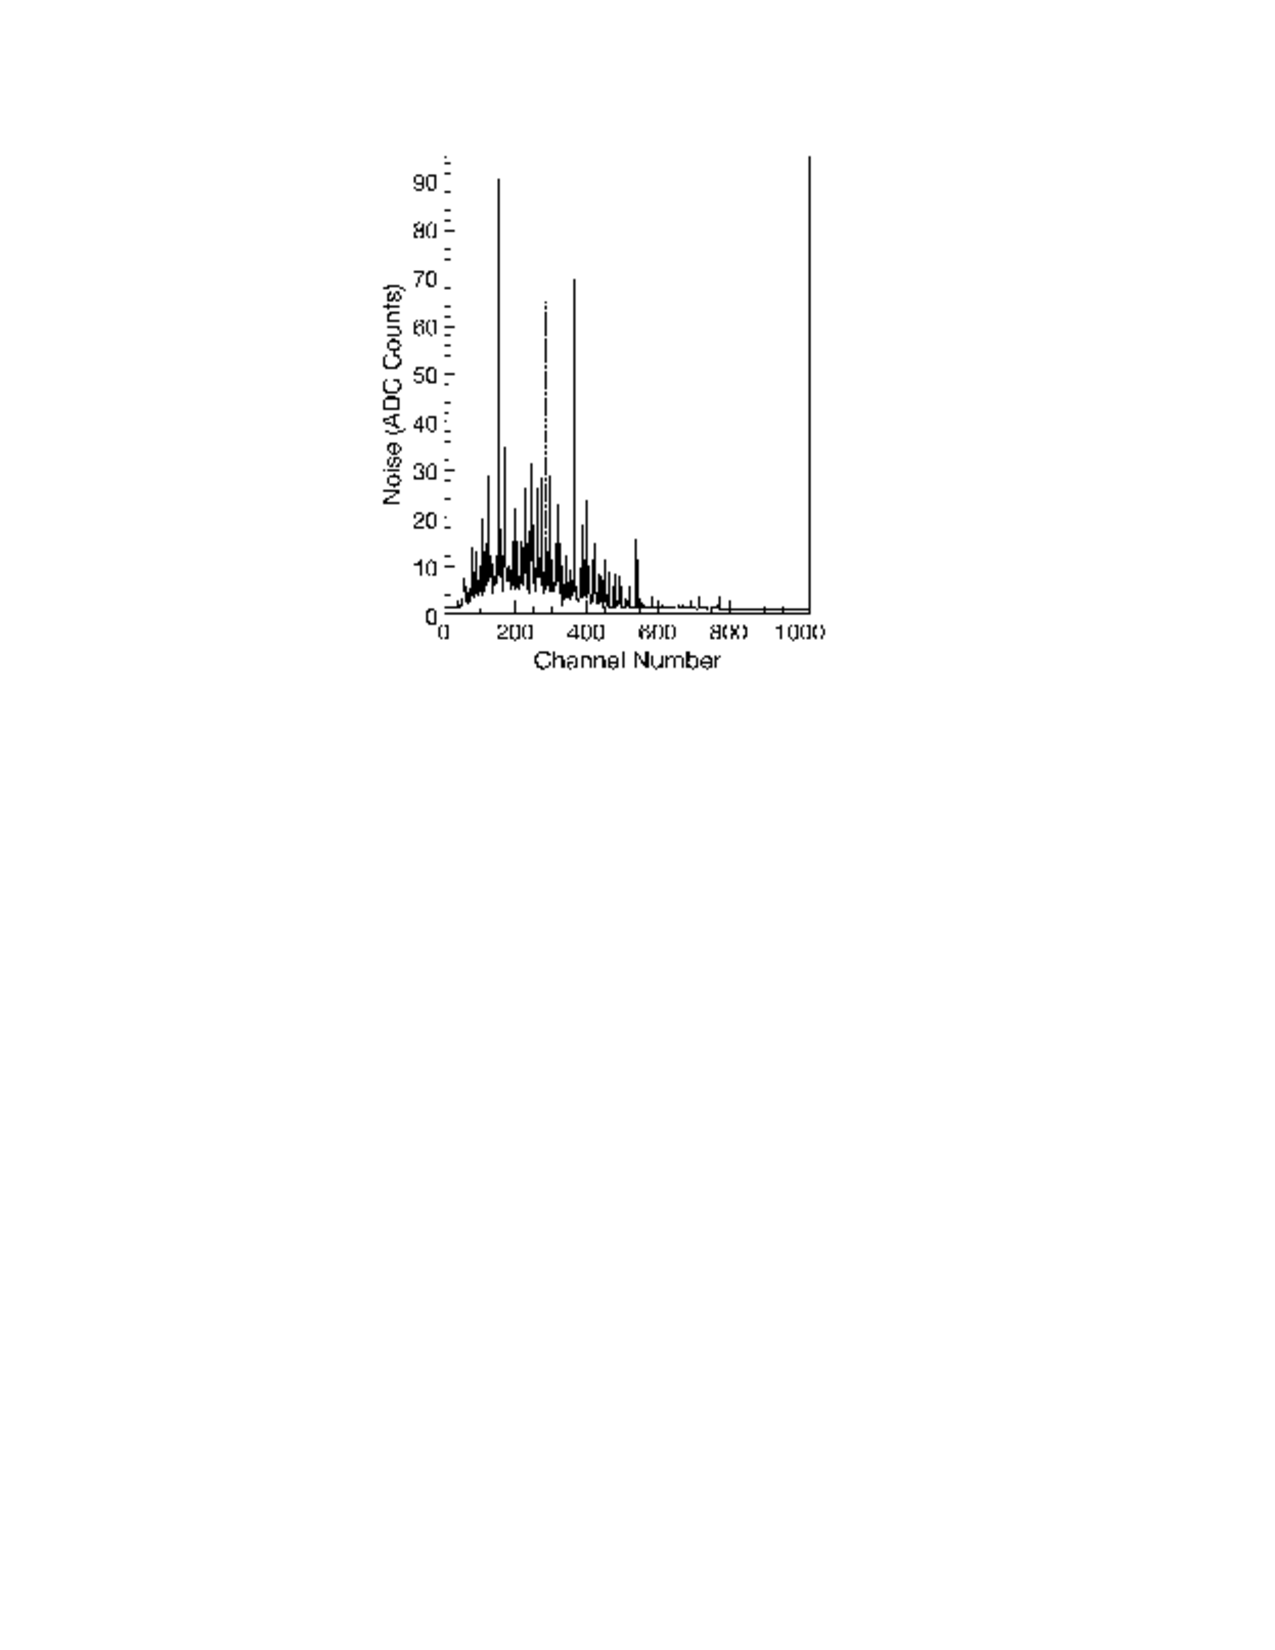
\includegraphics[height=0.4\textheight,
      width=0.45\textwidth]{./Images/11_SMT}
      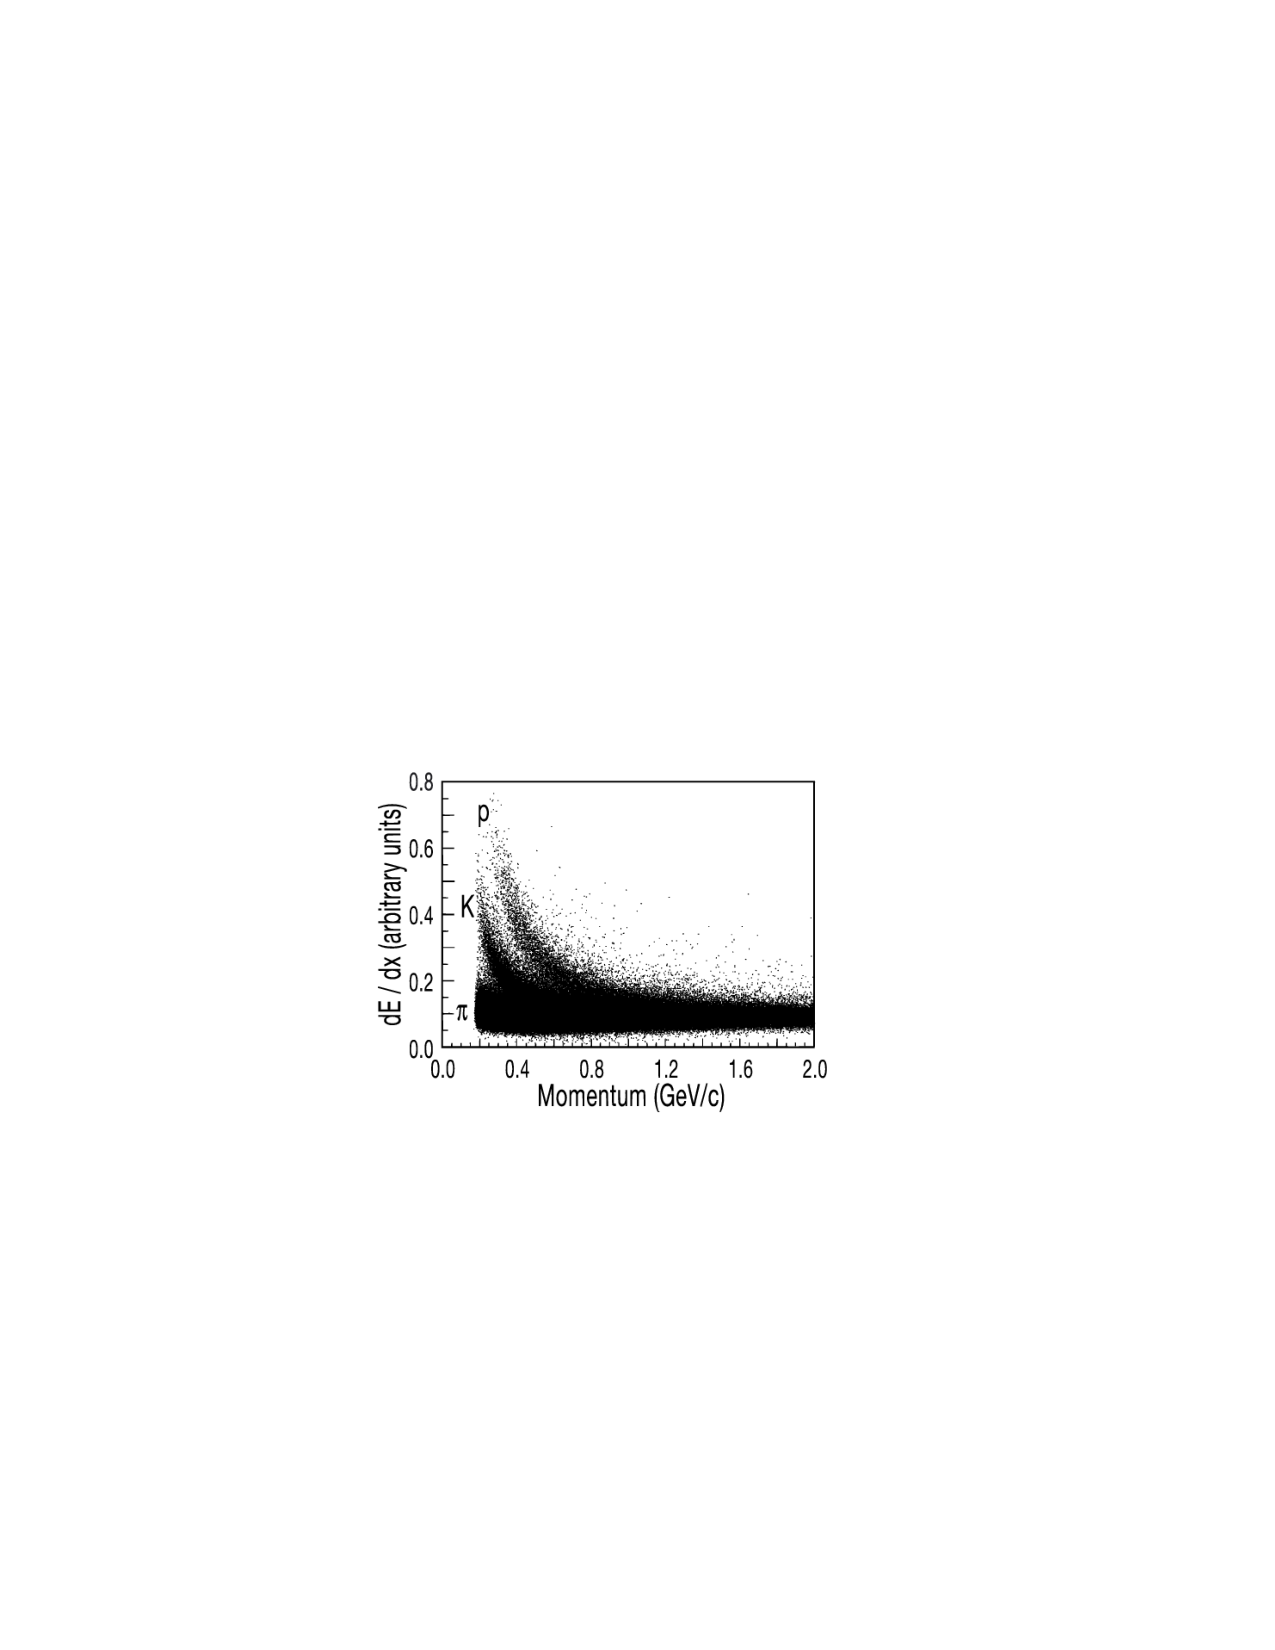
\includegraphics[height=0.4\textheight,
      width=0.45\textwidth]{./Images/12_SMT}
      \caption*{left: grassy noise seen in the Micron-supplied F-disk
        detectors. right: energy loss for a $K$-enriched sample of
        tracks showing $\pi$, $K$, and proton bands.}
      
    \end{figure}
    \itt[<only@+>]  
    
\item during run II $\approx 90$\% of sensors were functional
  
\item most operational difficulties have been peripheral to the
  silicon detector itself. These include latchup of operational
  amplifiers on the interface boards, low voltage power supply
  failures, and high leakage currents in high voltage distribution
  boxes.
  
  \note{\url{https://en.wikipedia.org/wiki/Latch-up}}
  
\item the most serious detector feature is “grassy noise,”
  which is confined to the Micron-supplied F-disk
  detectors ($75$\% of the F-disk sensors). This noise is characterized
  by large charge spikes which cover $10–20$ strips and
  occur in about $20$\% of the events for affected
  devices.
  
\item leakage currents typically rise to
  greater than $100 \mu A$ within one hour of turn-on at
  the beginning of a store.
  
\item Alignment and calibration Signal/noise performance varies with
  detector type from $12:1 to 18:1$.
  
\item Coherent noise is typically one-third
  of the random noise.
  
\item Gains vary among detector types
  with the n-sides $5–15$\% lower than the p-sides due to the larger load
  capacitance.
  \tti
  
\end{overlayarea}
\end{frame}


\subsection{Central fiber tracker}


%%%%%% SLIDE
\begin{frame}{\textcolor{Goldenrod}{Central Fiber Tracker}}
  \begin{overlayarea}{\textwidth}{\textheight}
    \begin{figure}[h]\centering
      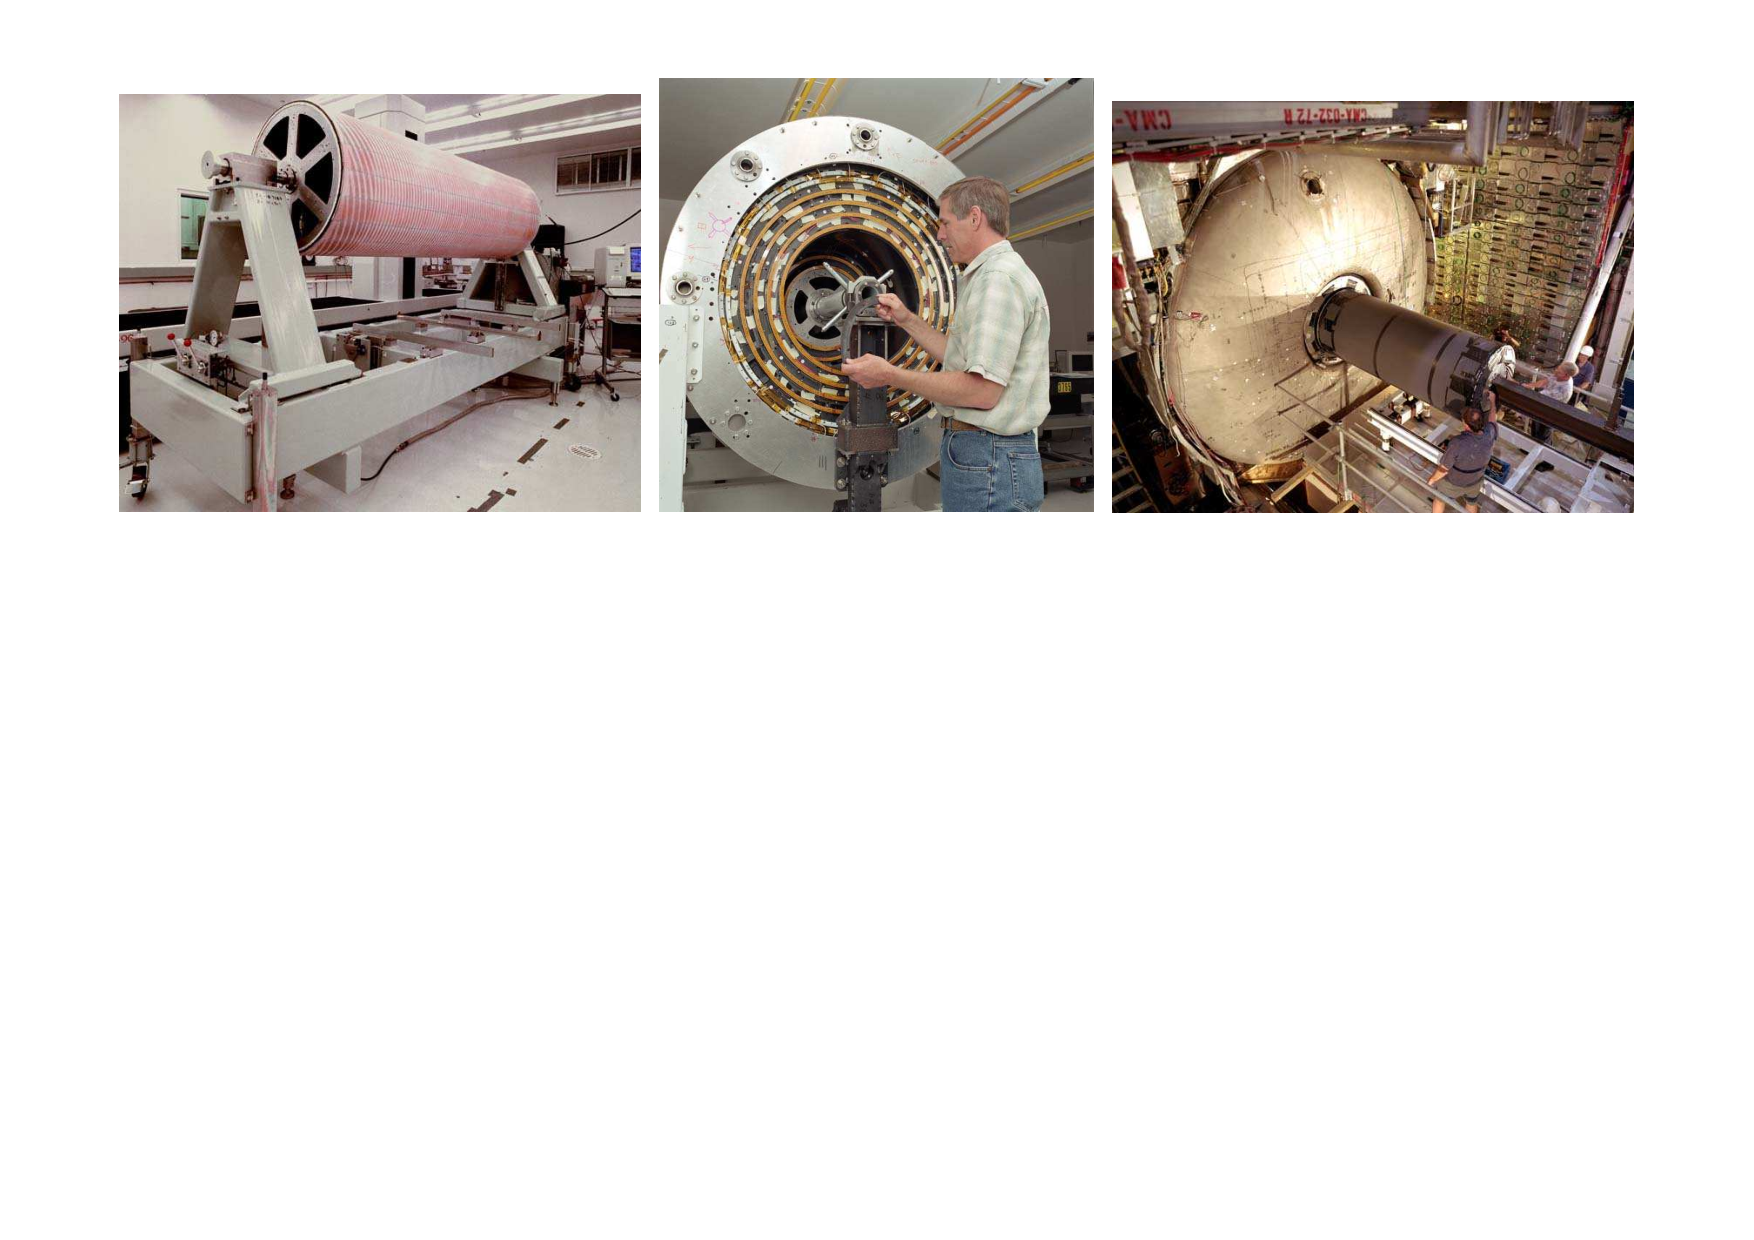
\includegraphics[height=0.3\textheight]{13_CFT}
    \end{figure}
    \itt[<only@+>]  

    \item The CFT consists of scintillating fibers mounted on eight concentric
      support cylinders and occupies the radial space from 20 to 52 cm from
      the center of the beampipe. To accomodate the forward SMT H-disks, the
      two innermost cylinders are 1.66 m long; the outer six cylinders are
      2.52 m long.
      
    \item 
      Each cylinder supports one doublet layer of fibers oriented
      along the beam direction (z) and a second doublet layer at a
      stereo angle in φ of +3◦ (u) or −3◦ (v).

    \item
      The scintillating fibers are coupled to clear fiber waveguides
      which carry the scintillation light to visible light photon
      counters (VLPCs, Section 2.2.4) for read out. The small fiber
      diameter (835 μm) gives the CFT an inherent doublet layer
      resolution of about 100 μm as long as the location of the
      individual fibers is known to better than 50 μm.
      

      
      \tti
\end{overlayarea}
\end{frame}

%%%%%% SLIDE
\begin{frame}{\textcolor{Goldenrod}{Central Fiber Tracker}}
  \begin{overlayarea}{\textwidth}{\textheight}
    \begin{figure}[h]\centering
      
    \end{figure}
    \itt[<only@+>]
    
    \tti
  \end{overlayarea}
\end{frame}


%%%%%% SLIDE
\begin{frame}{\textcolor{Goldenrod}{Central Fiber Tracker}}
  \begin{overlayarea}{\textwidth}{\textheight}
    \begin{figure}[h]\centering
      
    \end{figure}
    \itt[<only@+>]
    
    \tti
  \end{overlayarea}
\end{frame}


%%%%%% SLIDE
\begin{frame}{\textcolor{Goldenrod}{Central Fiber Tracker}}
  \begin{overlayarea}{\textwidth}{\textheight}
    \begin{figure}[h]\centering
      
    \end{figure}
    \itt[<only@+>]
    
    \tti
  \end{overlayarea}
\end{frame}


%%%%%% SLIDE
\begin{frame}{\textcolor{Goldenrod}{Central Fiber Tracker}}
  \begin{overlayarea}{\textwidth}{\textheight}
    \begin{figure}[h]\centering
      
    \end{figure}
    \itt[<only@+>]
    
    \tti
  \end{overlayarea}
\end{frame}

